\chapter{Implementation}
\label{cha:implementation}
\epigraph{What runs, the code or the comments?}{Brian Kernighan}

\noindent
The code.
With comments being non-executable meta information, Brian Kernighan's question has to be answered with: "the code".
\begin{itemize}
    \item But does it have to be this way?
    \item Is it possible to run comments?
    \item Does it make sense?
    \item Can we blur the lines?
\end{itemize}
As we have seen in Chapters~\ref{cha:introduction} and \ref{cha:related-work}, while the original idea of Hole-Driven Development is closely linked to statically typed functional programming languages, in this chapter we introduce \emph{Holey}\footnote{More information regarding usage and source code can be found at \url{https://holey.dev}.}, our approach on bridging the gap between the type-theoretic formal aspects of Hole-Driven Development and practically applying its ideas to widely used general-purpose programming languages.

\section{Types of Holes}
\label{sec:holey-types-of-holes}
Until this section, we divided our analysis between todo comments and holes or hole-like alternatives.
If we apply the analogy of a fill-in-the-blanks exercise to programming in general, we can conclude that there is little difference between todo comments, holes, and hole-like alternatives.
They are all blanks that have to be filled in.
But they are not the same; they do have different applications as well as different capabilities.
When we started working on applying hole-driven ideas to \CS at first, we created our own \emph{DSL} (domain-specific language) for writing holes.
After working with this DSL and comparing it with existing solutions and best practices, we quickly realized that while it enabled Hole-Driven Development, it was far off idiomatic \CS-code.
As we identified the idiomatic usage as one of the main properties of holes (compare \ref{hp:idiomatic}), we reverted this approach and examined how existing \CS-features can be re-used as holes.
In this section, we will introduce our classification of the most widely used and applicable types of holes while explaining their usage and use cases. 

\subsection{Todo-Comment}
As seen in Section~\ref{sec:introduction-about-todo-comments}, todo comments are widely used and supported \cite{jetbrains_todo_2023}.
By re-inventing them, legacy code could not be supported, and developers would have to learn a new concept or syntax.
Additional tools for managing todo comments as presented in Section~\ref{sec:tackling-todo-comments} would not be compatible as well.
Furthermore, todo comments are concise to write (\ref{hp:concise}), idiomatic to \CS (\ref{hp:idiomatic}), and allow developers to specify ideas in plain text (\ref{hp:prose-message}).

However, as asked by Brian Kernighan: "What runs, the code or the comments?"
Comments are not intended to be executed; they provide meta-information during development time but not at runtime.
As such, it is essential that they are not missed, which is enabled by emphasizing their existence at compile time (compare Section~\ref{sec:holey-roslyn-analyzers}, \ref{hp:compile-warnings}).
Although using approaches like source generators (compare Section~\ref{sec:source-generators}), they could actually influence the execution of a program; hence, they could be executed, Holey provides the abstraction of \emph{side effects} (compare Section~\ref{sec:hole-type-side-effect} for this kind of requirement.

Program~\ref{prg:holey-todo-comment} shows the usage of todo comments in \CS.
Nothing about their syntax or usage is specific to Holey.
However, if todo comments exist in a code base using Holey, they get reported as compiler warnings (compare Section~\ref{sec:providing-ide-support}) due to them being unaddressed.

\begin{program}[ht]
\begin{CsCode}
public interface ISidecarConnection
{
	// TODO: get rid of this initialize method; it should be in another interface
	void Initialize();
}
\end{CsCode}
\caption{Usage of a Todo Comment in Holey.}
\label{prg:holey-todo-comment}
\end{program}

\subsection{Hole-Comment}
The category of \emph{hole comments} is introduced based upon existing solutions regarding the usage of todo comments like PEP 350 -- Codetags or TagSea (compare Section~\ref{sec:tackling-todo-comments}).
By adding a configurable tag (\ref{hp:taggable}) in brackets after the todo-identifier, todo comments are interpreted as hole comments.
An example of this can be seen in Line~\verb|3| of Program~\ref{prg:holey-hole-comment} where adding \verb|[Refactor]| to the existing todo comment marks it as one that indicates a need for refactoring.
As described by \citeauthor{goldin_stop_2022}, if a todo comment indicates a certain action, it should be specified \cite{goldin_stop_2022}.
This enables developers to categorize todo comments and prioritize them.

At compile time, hole comments are reported using the "information" severity.
This decision was made because they already contain information about how they should be handled.
We hypothesize that this distinction also helps when converting legacy code bases, because by addressing the warnings raised by todo comments one by one, they can be either left as todo comments, enhanced with additional information for handling them later, or directly addressed by getting rid of them.

\begin{program}[ht]
\begin{CsCode}
public interface ISidecarConnection
{
	// TODO [Refactor]: get rid of this initialize method; it should be in another interface
	void Initialize();
}
\end{CsCode}
\caption{Usage of a Hole Comment in Holey.}
\label{prg:holey-hole-comment}
\end{program}

\subsection{Missing Implementation}
As Section~\ref{sec:simulating-holes} explains, \texttt{NotImplementedException} is an exception class in \CS's standard library that denotes some implementation is still under development.
Program~\ref{prg:holey-notimplemented} shows the usage of the \texttt{NotImplementedException} where on Line~\verb|6| the default case in a switch-expression is denoted as not implemented.
By not handling all cases, the software\footnote{In this case, the software is Holey itself, which we also develop using the hole-driven approach enabled by Holey.} can already be executed and tested without the need of handling all edge cases.
Not handling edge cases works during development but will probably crash at runtime.
Although IDEs such as Rider show usages of \texttt{NotImplementedException} in the todo window \cite{jetbrains_todo_2023}, they do not surface at compile time.
Similar to todo comments, Holey makes \texttt{NotImplementedException}s visible at compile time by reporting their usages as warnings.
We chose "warning" as the severity for throwing a \texttt{NotImplementedException} because although the program can be run, it will crash once a non-implemented program path is encountered.

\begin{program}[ht]
\begin{CsCode}
holeInformation switch
{
	HoleInformation.EmptyEffect emptyEffect // ...
	HoleInformation.Value value => // ...
	HoleInformation.Effect effect => // ...
	_ => throw new NotImplementedException(\$"{holeInformation.Type} is not handled")
}
\end{CsCode}
\caption{Usage of \texttt{NotImplementedException} in Holey.}
\label{prg:holey-notimplemented}
\end{program}

\subsection{Side-Effect}
\label{sec:hole-type-side-effect}
In addition to supporting idiomatic, built-in \CS features, Holey adds the notation of side effect holes.
They correspond most closely to the original definition of holes by resembling executable (\ref{hp:executable}) parts of source code, whose runtime behavior (\ref{hp:runtime-behavior}) can be specified while being further described by a textual message (\ref{hp:prose-message}).
Side-effect holes can be seen as abstract I/O (input and output), which makes them Holey's most powerful abstraction.

Their usage is shown in Program~\ref{prg:holey-side-effects}.
Every value that enters an application and every action that somehow changes the outside world is a side-effect.
After multiple rewrites and simplifications we realized that providing a way to get some value and providing another way to execute an effect is enough to model arbitrary runtime behavior in holes.
As such, a side-effect hole can be introduced using the static method \verb|Hole.Todo(...)|.

By providing a uniform static method to introduce side-effect holes we managed to create a concise notation (\ref{hp:concise}) that also allows holes to be nestable (\ref{hp:nestable}).
As shown in Line~\verb|1| of Program~\ref{prg:holey-side-effects}, Holey has to be imported before it can be used which is limited by the way \CS works, but modern IDEs automatically suggest such usings and \CS 10 enables imports to be defined only once using Global Usings \cite{koch_global_2021}.

\begin{program}[ht]
\begin{CsCode}
using Holey;

var number = Hole.Todo("generate a random number", 42);
var apiKey = Hole.Todo(
	"read the API_KEY from our configuration management service",
	() => Environment.GetEnvironmentVariable("API_KEY")
);
Hole.Todo("validate the incoming data");
await Hole.Todo("save the form data asynchronously", Task.Delay(500));

record User(string Name, int Age);
var user = Hole.Todo("load user data", value => value.Prompt<User>());
\end{CsCode}
\caption{Usage of side-effects in Holey.}
\label{prg:holey-side-effects}
\end{program}

As shown in Program~\ref{prg:holey-side-effects}, the first parameter of \verb|Hole.Todo(...)| is a string.
This string acts as the hole's description and lets developers use the informal nature of textual descriptions to describe the intent of the hole.
The second parameter is optional and provides a temporary implementation for the hole.
The type of this second parameter, distinguishes between a hole that provides a value (if \verb|T| is returned) and a hole that executes an effect (if \verb|void| is returned).
This second parameter also distinguishes multiple overloads of the static method \verb|Hole.Todo(...)| whose differences are explained in the rest of this section.

\subsubsection{Values and Effects}
Side-effect holes can either provide a value or execute some effect.
This differentiation is based on whether the hole returns something.
Lines~\verb|3-7| and \verb|12| of Program~\ref{prg:holey-side-effects} show how values can be provided using holes.
If the second parameter is either a constant value or a function returning a value, the hole provides this value, by either simply returning the constant or executing the function and return its result.
Lines~\verb|8| and \verb|9| of Program~\ref{prg:holey-side-effects} depict the usage of effects.
Both statements do not return anything.
The hole in Line~\verb|8| does not take a second parameter, which indicates that something (the task described as the first parameter) has yet to be done.
In comparison to a todo comment, this side-effect hole can be inspected at runtime (compare Section~\ref{sec:reporting}).
The hole in Line~\verb|9| simulates the asynchronous saving of some form data.
Similar to the value holes it simply wraps the task, awaits it, and enhances it with reporting functionality.

One might wonder what is novel about wrapping values and functions and simply returning or calling them.
Wrapping them makes them inspectable at compile-time and runtime, which enables Hole-Driven Development using IDE integrations (compare Section~\ref{sec:providing-ide-support}, runtime reporting (compare Section~\ref{sec:reporting}) and extensibility.

\subsubsection{Asynchrony and Laziness}
As visible in Line~\verb|9| of Program~\ref{prg:holey-side-effects}, holes can be made asynchronous and therefore have to be awaited.
This can simply be accomplished by passing \verb|Task<T>| or \verb|Task| as the second parameter, where the former results in a hole that provides a value, where the latter simulates an effect.
Another aspect of side-effect holes is their laziness.
If the hole's temporary content shall be evaluated lazily, a function can be passed as the secondary parameter which is only evaluated once the hole gets executed.
Laziness and asynchrony can also be combined which enables asynchronous holes that are evaluated lazily.

\subsubsection{Extensibility}
One of the features that makes Holey and its side-effect holes so powerful is its extensibility.
Line~\verb|12| of Program~\ref{prg:holey-side-effects} shows how side-effects can be extended.
Both values and effects can be provided by extension methods.
The method \verb|Prompt<T>()| in Line~\verb|12| shows such an extension by prompting for a user via Holey's Sidecar (compare \ref{sec:holey-sidecar}) application.
These extension can be defined as custom \CS-libraries and allow Holey to be customized for specific use-cases.


\section{Architecture}
\label{sec:holey-architecture}
At its core Holey is a \CS-library which is supported by .NET-analyzers (compare Section~\ref{sec:holey-roslyn-analyzers}).
To improve learnability and backwards-compatibility, these analyzers support the inspection of todo comments as well as usages of \verb|NotImplementedException|.
In addition to those, the analyzers also report usage information about the holes provided by the library as well as configurable usage of hole comments.
This library and its accompanying analyzers are supported by a Visual Studio extension and an external Sidecar application.
The Visual Studio extension bridges the analyzer results reported by Holey to Visual Studio's task list.
This guarantees that familiar development practices can be continued and shows how extension for additional integrated development environments can be created.
The Sidecar application extends Holey's side-effect holes with additional runtime features.
It is written as a web application which can connect to the Holey library via different communication channels (e.g., Websockets, \verb|postMessage|-function of iFrames) and display information about the usage of holes as well as interact with the application under development via interactive holes.
It also acts as an example of how Holey can be extended and Hole-Driven Development in general-purpose programming languages can lead to interactive programming.

Figure~\ref{fig:holey-architecture} depicts the interaction between these components visually.
\begin{figure}[ht]
    \centering
    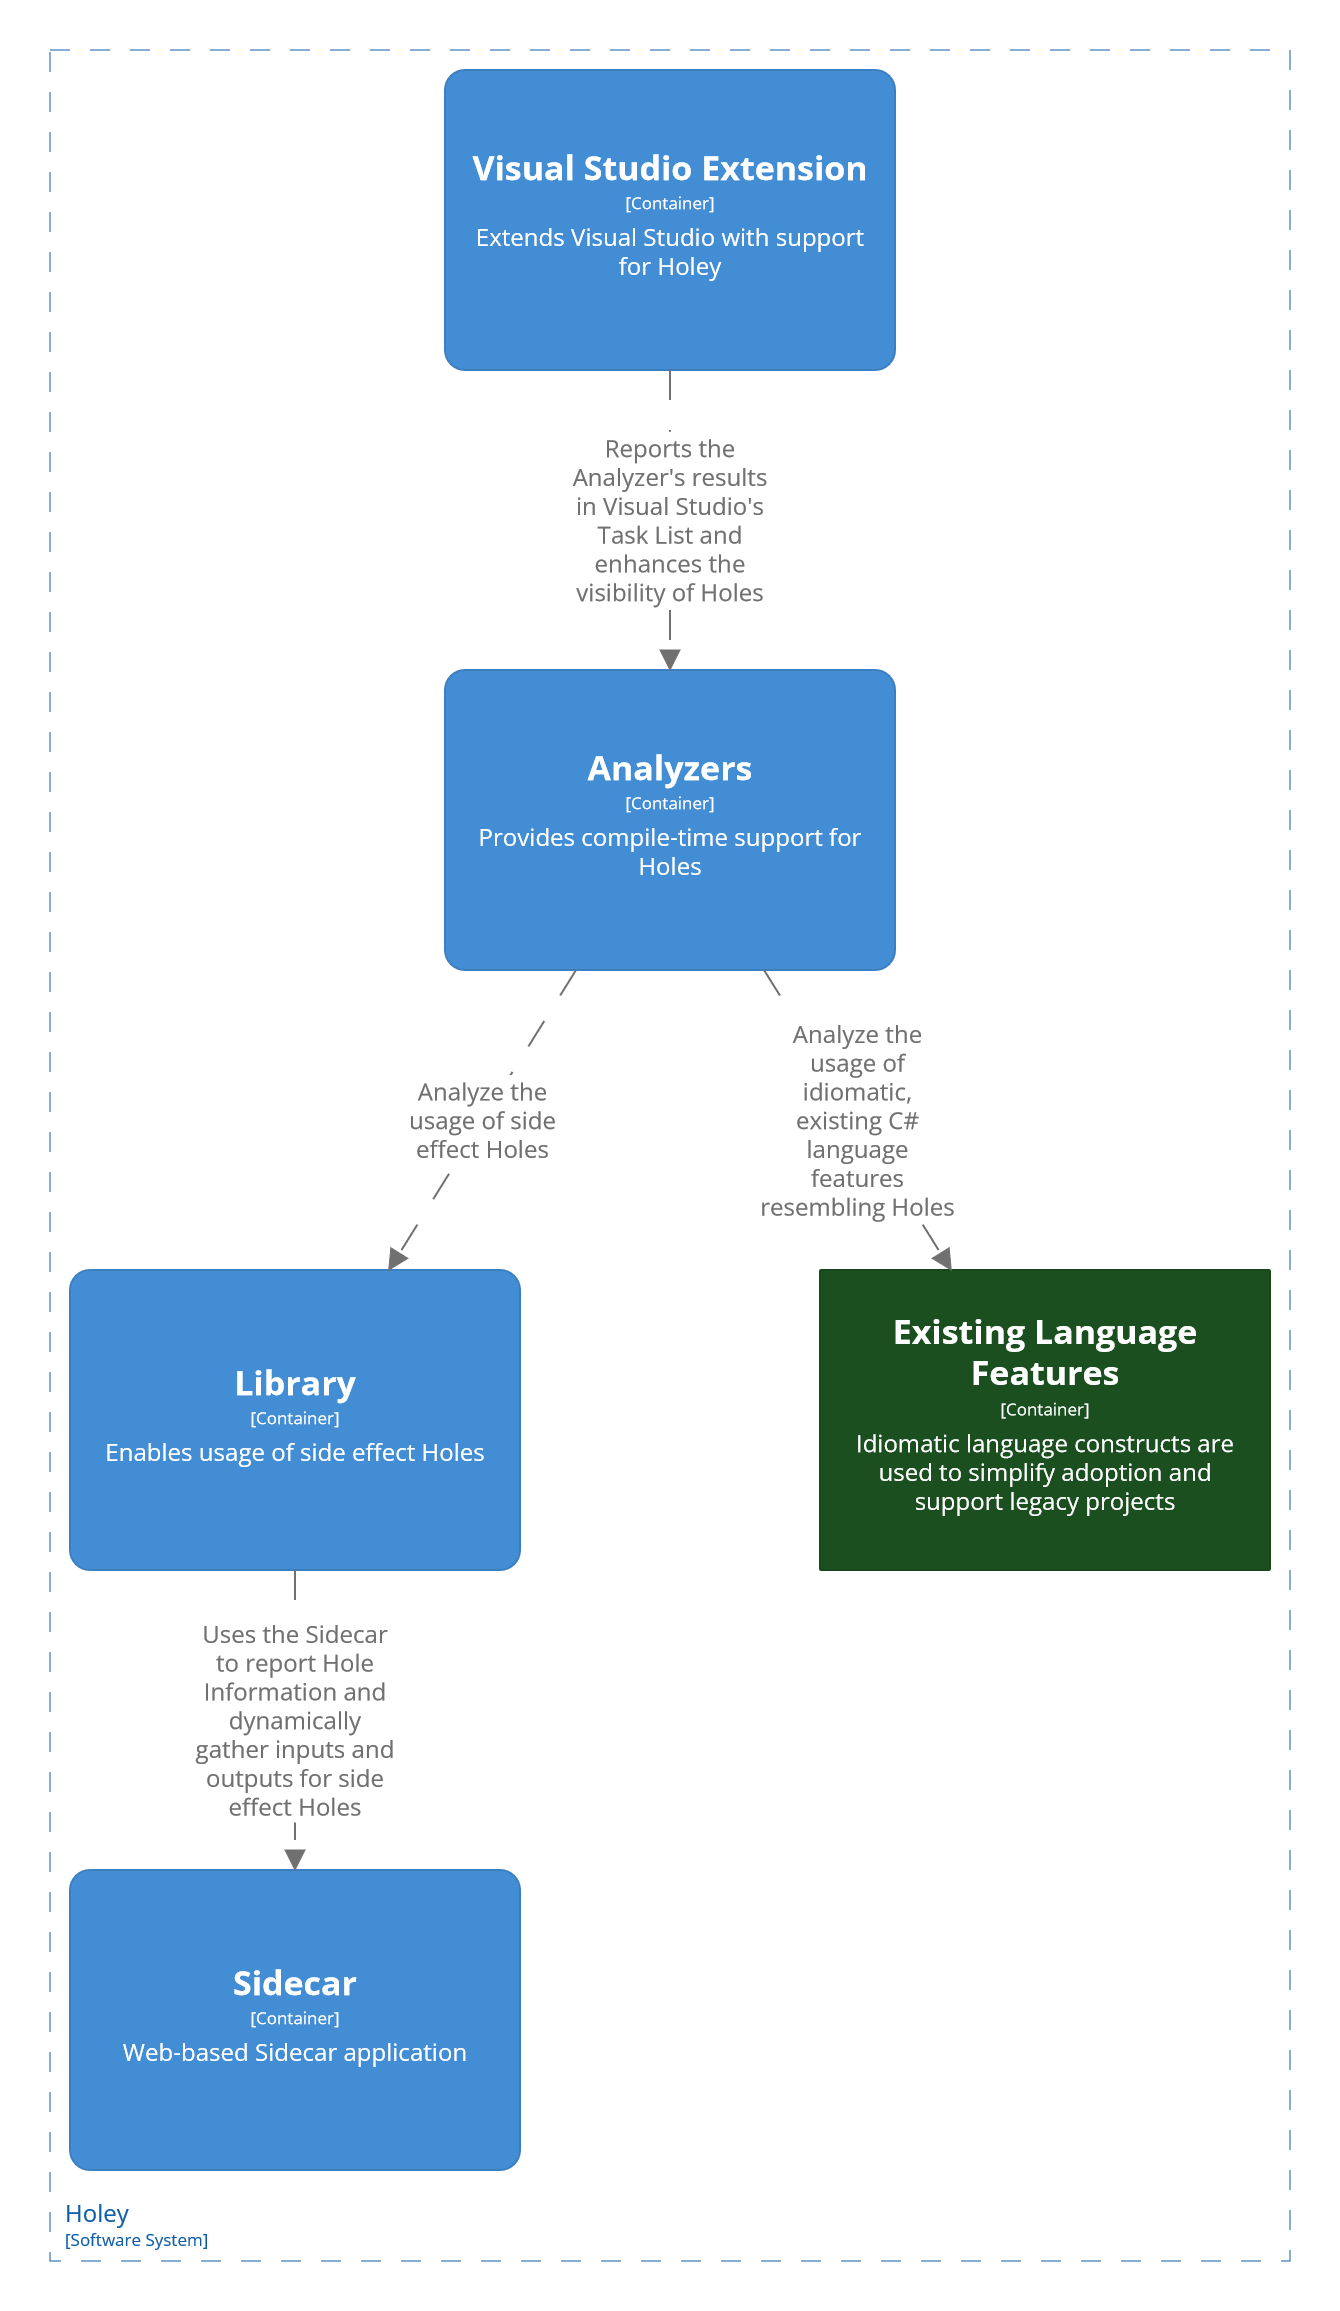
\includegraphics[width=0.97\textwidth]{images/holey-architecture}
    \caption{Overview of the main components of Holey modeled using C4.}
    \label{fig:holey-architecture}
\end{figure}

\subsection{Enabling Configuration}
\label{sec:holey-enabling-configuration}
As explained in Section~\ref{sec:hole-type-side-effect}, Holey provides side-effect holes which affect the runtime behavior of the software under development.
According to \ref{hp:executable} and \ref{hp:runtime-behavior} runtime behavior affecting holes should be configurable.
As such, Holey provides multiple ways of configuration, depicted in Program~\ref{prg:holey-enabling-configuration}:
\begin{itemize}
    \item The library supports logging via standard .NET logging interfaces (compare Section~\ref{sec:holey-supporting-logging}). This allows consumers to log information originating from Holey to be either logged with the rest of the application's logging concerns or completely separately.
    \item Hole supports reporting (compare \ref{sec:reporting}) which can be used to inspect holes at runtime. E.g., users of Holey could display toast notification for discovered holes. This allows incomplete applications to be started (\ref{hp:executable}), but highlights their lacking functionality at runtime.
    \item Holey offers multiple extensibility points. Developers can e.g., create custom side-effect holes that get their input from mocked dummy systems; allow such input to be serialized as inputs for tests or create custom re-usable reporting user interfaces.
\end{itemize}

\begin{program}[ht]
\begin{CsCode}
Holes
	.UseLoggerFactory(/*...*/)
	.UseReporting(/*...*/)
	.UseExtensions(/*...*/);
\end{CsCode}
\caption{Configuring the runtime behavior of Holey.}
\label{prg:holey-enabling-configuration}
\end{program}

One difficulty that arose from designing the syntax for side-effect holes as concise as possible was the failing support for dependency injection when using static methods.
This makes it harder to create an extensible library.
We overcome this problem by using a static instance of a dependency injection container which provides the necessary dependencies for extensions and can be configured differently when testing the library.

\subsection{Supporting Logging}
\label{sec:holey-supporting-logging}
Microsoft provides a common abstraction for logging built around the \verb|ILogger|-interface \cite{microsoft_logging_2023}.
They define three interfaces with different responsibilities \cite{bahreini_should_2018}:
%
\begin{description}
    \item[\texttt{ILogger}] This interface abstract functionality for writing a log message of a given \emph{Log Level}.
    \item[\texttt{ILoggerProvider}] Providers are responsible for creating \verb|ILogger| instances. They are not supposed to be used directly.
    \item[\texttt{ILoggerFactory}] One or more logging providers can be registered with a logging factory, which in turn uses all of those providers when creating an \verb|ILogger| instance.
\end{description}

For using these interfaces in dependency injection, Microsoft recommends two different ways \cite{microsoft_logging_2023}.
One can either inject \texttt{\seqsplit{ILoggerFactory}} and use its \texttt{\seqsplit{CreateLogger(string <category>)}}-method or directly inject a typed \texttt{\seqsplit{ILogger<T>}} instance.
Both methods are responsible for setting the logger's category to the fully qualified class name of the class it is used in.
However, injecting a \texttt{\seqsplit{ILoggerFactory}} violates the single responsibility principle \cite{bahreini_should_2018} because a class should not be responsible for creating its own logger.
Injecting the fully qualified \texttt{\seqsplit{ILogger<T>}} instance adds unnecessary noise.
Theoretically, a class should depend on the non-generic interface \texttt{\seqsplit{ILogger}} while its class name is set as its category.

Program~\ref{prg:holey-supporting-logging} shows how we solved this problem.
We are using Stashbox\footnote{\url{https://z4kn4fein.github.io/stashbox/}}, a lightweight, fast, and portable dependency injection framework for .NET for injecting dependencies throughout Holey.
In Line~\verb|1| we register the non-generic \verb|ILogger| interface and use the parent's type information (compare Lines~\verb|6| and \verb|10|) to set the logger's category when creating it via the configured logger factory.
By using this approach, classes can expect an instance of \verb|ILogger| with the pre-configured category while the dependency resolution throws an exception if an instance of \verb|ILogger| is requested outside of a class scope.

\begin{program}[ht]
\begin{CsCode}
Container.Register<ILogger>(
	config =>
		config
			.WithFactory<TypeInformation>(
				typeInfo =>
					typeInfo.ParentType is null
						? throw new InvalidOperationException(
							\$"An ILogger can only be injected into a class, because it uses this class' FullName as its scope."
						)
						: loggerFactory.CreateLogger(typeInfo.ParentType.FullName)
			)
			.ReplaceExisting()
);
\end{CsCode}
\caption{Using the Stashbox dependency injection framework to provide properly configured \texttt{ILogger}-instances to Holey's extensions.}
\label{prg:holey-supporting-logging}
\end{program}

\subsection{Enabling Language Independence}
\label{sec:holey-enabling-language-independence}
During the multiple rewrites, we realized that simplifying the concept of Hole-Driven Development to a few simple primitives provides another impactful advantage: language independence.
Holey's underlying concept is not tied to a specific programming language at all.
Although we conducted our proof-of-concept implementation in \CS, supporting other languages should be possible.
Adopting Holey's interpretation of Hole-Driven Development in other languages requires these functionalities:

\begin{description}
    \item[Todo Comments] By re-using todo comments, we created an idiomatic and backward-compatible solution regarding the most basic form of adapting holes. If a language supports comments and somehow allows them to be tagged as \emph{to be done}, it supports todo comments.
    \item[Exceptions] Simulating empty holes is accomplished by throwing an exception. If a concept like \CS's \verb|NotImplementedException| already exists in a language, it should be re-used; otherwise, a custom exception type could be defined.
    \item[Custom Control Structures] Supporting side-effect holes requires the language to be somehow extendable; defining a function is enough. If this function should interact with some external tool, some way of I/O is necessary. Integration with Holey's Sidecar application is simplified a lot if there are existing libraries for handling JSON Schema and Websocket connections.
    \item[Linters] One of the vital parts of Hole-Driven Development is compile-time information on holes. This can be achieved by compiler plug-ins, as shown in our proof-of-concept, or even in non-compiled languages by static code analysis. One such solution could be the definition of custom linting rules highlighting the usage of holes.
\end{description}

\section{Providing IDE Support}
\label{sec:providing-ide-support}
As analyzed in Section~\ref{sec:languages-with-native-holes-support}, one crucial property of holes is that they generate warnings or errors at compile time (\ref{hp:compile-warnings}), which increases their visibility during development and allows them to be used as checklists.
%
\begin{figure}[ht]
    \centering
    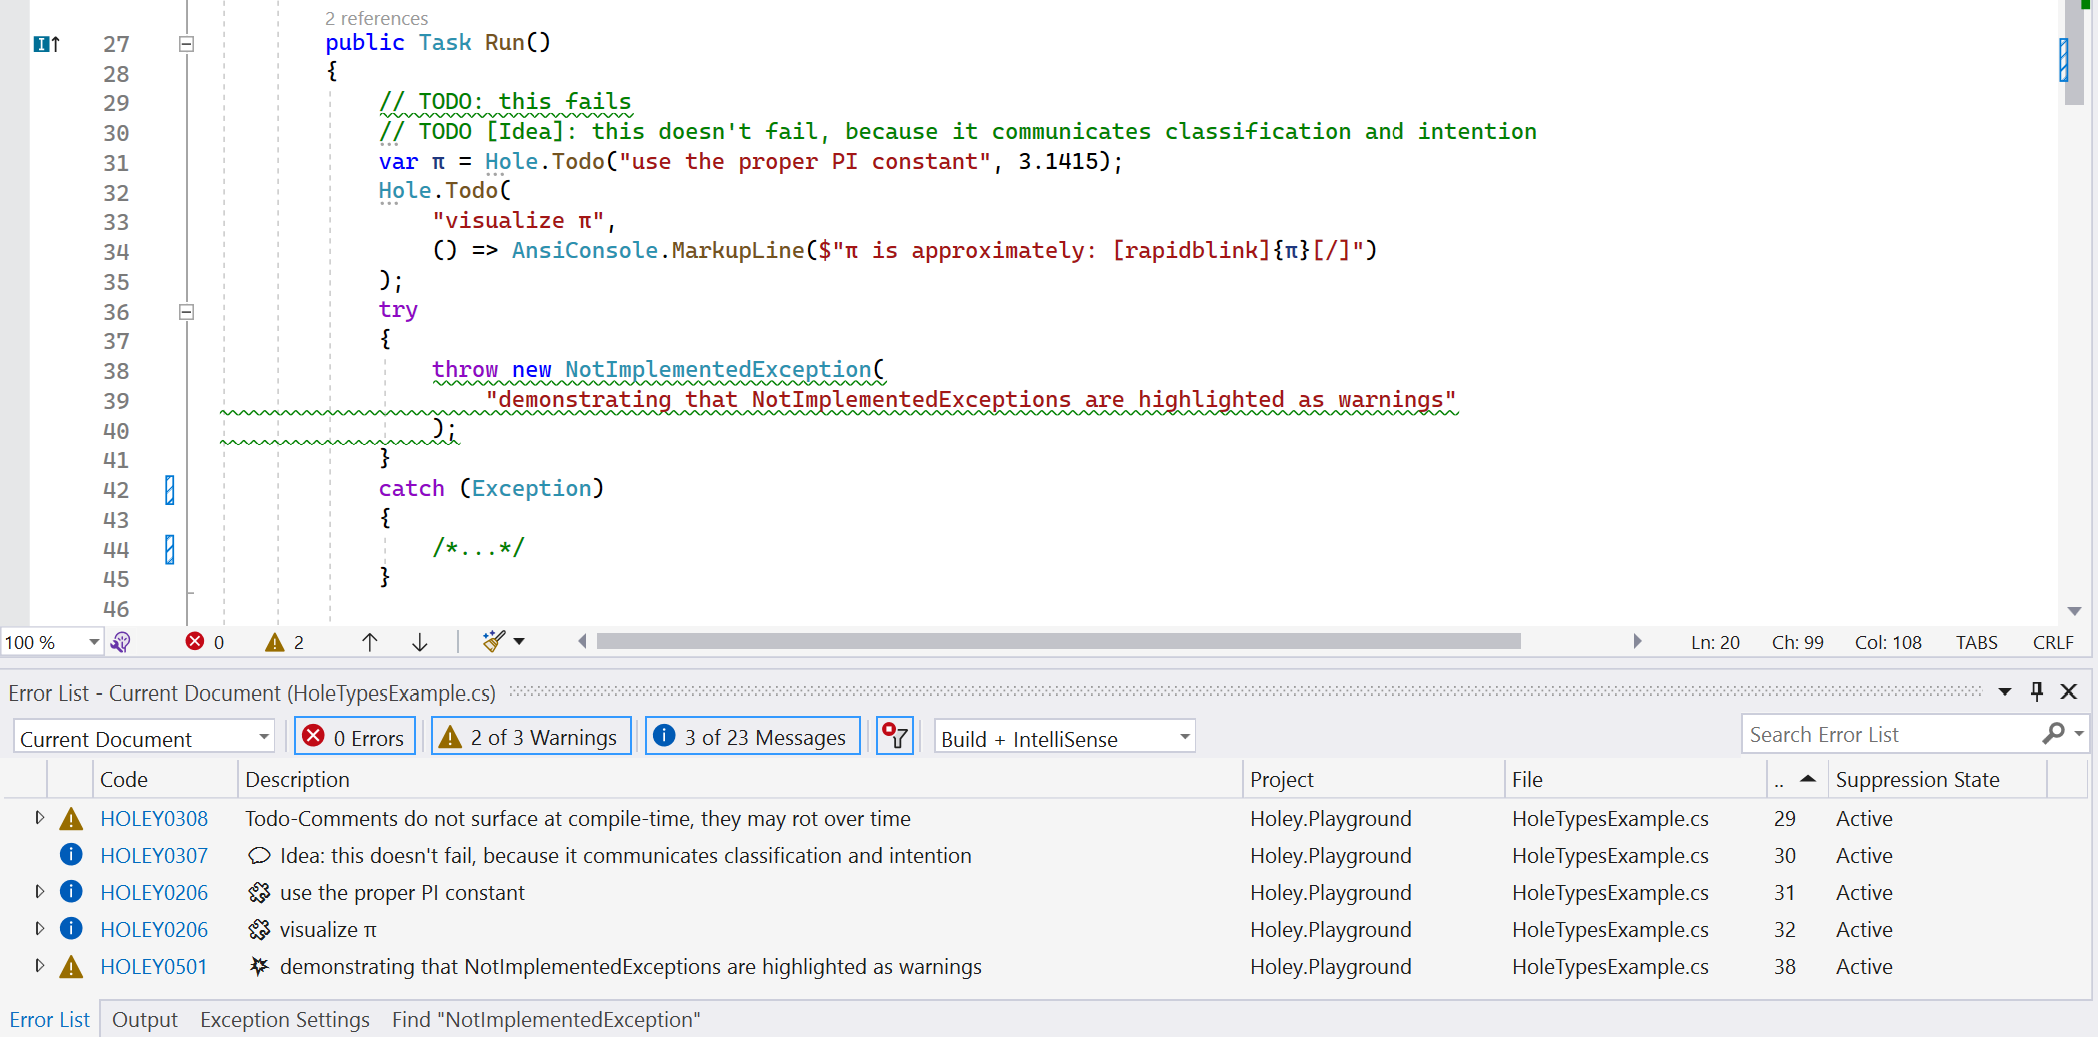
\includegraphics[width=0.97\textwidth]{images/ide-reporting}
    \caption{Usage of Holey in Visual Studio. The IDE provides proper error reporting in the source code itself and in Visual Studio's Error List.}
    \label{fig:providing-ide-support}
\end{figure}
%
Figure~\ref{fig:providing-ide-support} depicts Holey's support for compile time hole reporting.
Its upper part shows the usage of the hole types described in Section~\ref{sec:holey-types-of-holes}.
While the todo comment and the thrown \verb|NotImplementedException| are underlined, the hole comment and the side effect holes are only indicated by three small grey dots below them.
This difference in their visual indication is explained by looking at the bottom part of Figure~\ref{fig:providing-ide-support}.
This panel shows Visual Studio's Error List, which provides more information about the holes, such as their severity, code, and description.
As explained in Section~\ref{sec:holey-types-of-holes}, different types of holes are reported with different severities (information vs warning).
The code identifies a particular type of hole, and its suffix is modeled semantically after the HTTP status codes \cite{mozilla_http_2023}.
The description either reports some information on what to change (in the case of the todo comment) or resembles the hole's description prefixed by an icon denoting the hole's type.
This allows the Error List to be used as a checklist, which gets created automatically based on the program's holes.

\subsection{Roslyn Analyzers}
\label{sec:holey-roslyn-analyzers}
The screenshot in Figure~\ref{fig:providing-ide-support} shows Holey's usage in \emph{Microsoft Visual Studio Community 2022} without additional plug-ins.
This is enabled using Roslyn \emph{analyzers} \cite{microsoft_code_2023}.
Roslyn is the name of the .NET Compiler Platform, which allows developers to write compiler integrations called Analyzers that inspect \CS\ or Visual Basic code for style, quality, maintainability, design, and other issues.

By directly integrating such analysis features into the compiler platform, different IDEs are automatically supported (\ref{hp:editor-independence}).
Analyzers allow developers to inspect the source code and report diagnostics that become compiler errors.

Depending on the configured build mode, we report different diagnostic severities in Holey (\ref{hp:severity-modes}).
This allows the application to be tested and prototyped in debug mode, but once release mode is enabled, warnings are issued for all still existing holes.
If we directly raise errors, we would rule out use cases where holes are intended to be in a release build.
As such, raising warnings can be combined with the \CS\ compiler flag \verb|TreatWarningsAsErrors| \cite{microsoft_c_2023}, which, as its name suggests, turns warnings into errors and should be enabled for proper release builds.

Another property of holes that can be (partially) supported by analyzers is the heavy usage of types to guide their implementation (\ref{hp:matchable-via-types}).
Roslyn analyzers provide the semantic model of the analyzed application which can be used to get information about its \emph{meaning}.
Figure~\ref{fig:reporting-types} shows our proof-of-concept in this regard.
Based on the hole's scope we query all possible variables and methods as well as their types.
As we also know the hole's expected type (compare Section~\ref{sec:source-generators}), we could combine these information and use it towards basic suggestions for program synthesis.
Apart from proving that it is technically possible, we did not pursue these efforts any further as it would have expanded the scope of this thesis too much.

\begin{figure}[ht]
    \centering
    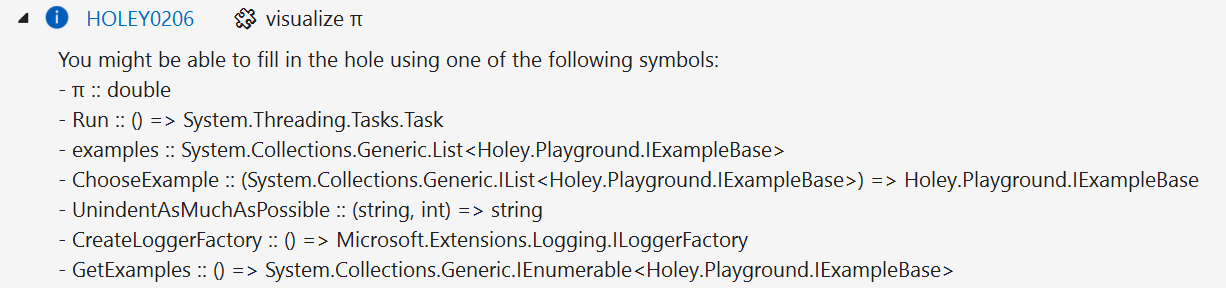
\includegraphics[width=0.8\textwidth]{images/reporting-types}
    \caption{Extracting Type Information from Holes to proof the Possibility of adding Program Synthesis.}
    \label{fig:reporting-types}
\end{figure}

\subsection{Code Fixes}
\label{sec:holey-code-fixes}
Based on analyzers (compare Section~\ref{sec:holey-roslyn-analyzers}), Roslyn provides another powerful, editor-independent feature called \emph{code fixes}.
By providing a code fix for a reported diagnostic, IDEs can suggest an automatic rewrite of the violating code.
Using this feature, it is possible to provide editor actions (\ref{hp:supported-editor-actions}) that are again editor independent (\ref{hp:editor-independence}).

\begin{figure}[ht]
    \centering
    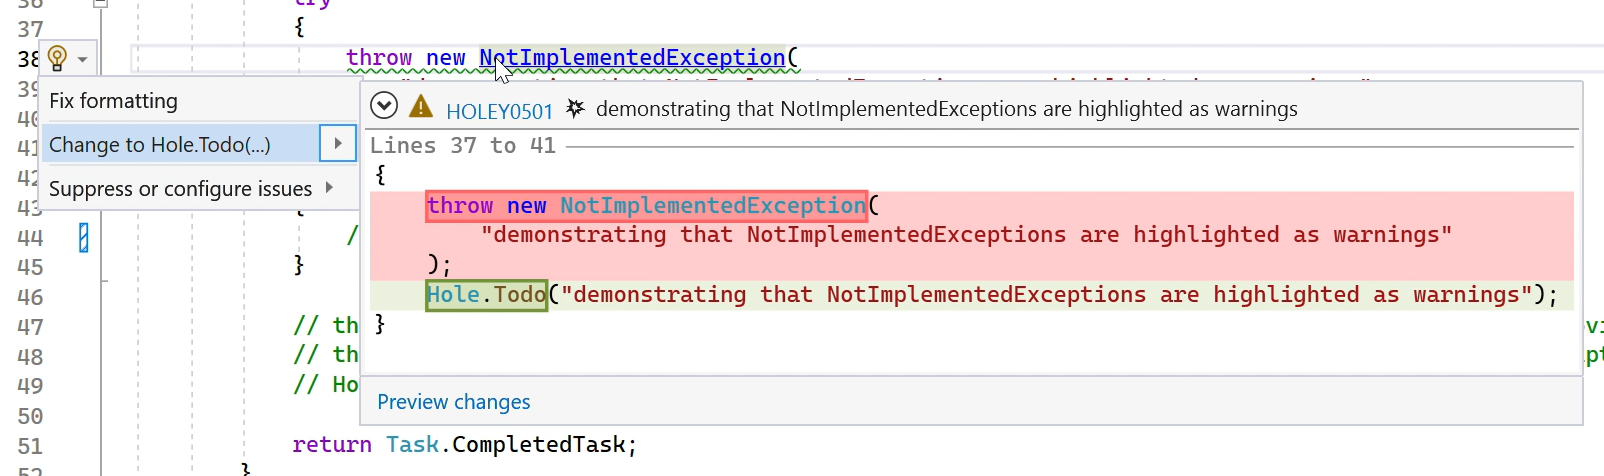
\includegraphics[width=0.9\textwidth]{images/code-fixes}
    \caption{Showcasing how Roslyn's Code Fixes are used to enhance the Editing Experience of Holes.}
    \label{fig:holey-code-fixes}
\end{figure}

Figure~\ref{fig:holey-code-fixes} shows these code fixes in action.
By pressing "Ctrl + .", Visual Studio provides its lightbulb suggestions, they can also be activated by clicking on the lightbulb in the left margin.
As it can be seen in Figure~\ref{fig:holey-code-fixes}, activating these suggestions opens an overlay which shows the difference between the existing code and the suggested fix.
Additionally to the analyzers we developed code fixes where applicable.
E.g., in the case of \verb|NotImplementedException| this enables developers to automatically convert them to side effect holes, without having to perform tedious text manipulations by hand.
Such code fixes have also been developed for converting todo comments and removing holes while replacing them with their current implementation.

\section{Bridging Compile- and Runtime}
\label{sec:holey-bridging-compile-and-runtime}
Holes can be seen as a bridge between compile time and runtime.
They provide information about their existence while developers are writing code and enable additional functionality (at least their inspection) at runtime.
This enables interesting extension capabilities (compare Section~\ref{sec:holey-extensibility}), but introduces the interesting challenge of how to gather information about the source code at runtime.
In this section we describe how we are able to gather information that is of interest to us, such as:
\begin{description}
    \item[Description] The textual description of the hole is a string literal. Ideally it explains why the hole exists or how it should be implemented. At compile time it is interesting to know the description for reporting diagnostics which allow the creation of checklists and at runtime it might be interesting to report holes as they are executed.
    \item[Location] The location of a hole is used to identify it and consists of its filename, line- and column number. It can also be used to create tooling which links to the holes and acts upon them.
    \item[Type] The type of a hole enables different visualization and interaction capabilities for tools.
    \item[(Expression)] Only side effect holes do have expressions. They represent the optional second parameter of side effect holes and can be empty in the case of an empty effect. Information about this expression can be visualized or used in extensions. It also lays the foundation for future tooling that might be built upon Holey (compare Section~\ref{sec:discussion-applications}).
    \item[(Return Type)] Only side effect holes that provide values do have a meaningful return type. It can also be visualized, used for extensions and provides the basis for program synthesis, as described in Section~\ref{sec:holey-roslyn-analyzers}.
\end{description}

\subsection{Compiler Info Attributes}
\label{sec:holey-compiler-info-attributes}
The \CS-compiler provides multiple attributes for determining caller information of methods \cite{microsoft_attributes_2022}.
These attributes can be applied to method parameters and the compiler automatically inserts literals as their default values into the \emph{Intermediate Language}.
This behavior prevents those attributes from being affected by obfuscation.
Parameters, where these attributes are applied, have to be optional and match their corresponding types.
According to Microsoft, the information provided by those attributes helps with tracing, debugging, and helps to create diagnostic tools.
As holes can be seen as diagnostic tools, using these attributes allows us to use compile time information at runtime, as Program~\ref{prg:holey-compiler-info-attributes} shows.
The method signature, depicted in Program~\ref{prg:holey-compiler-info-attributes}, is taken from the simplest form of a value providing side effect hole which returns a variable or a literal.
By applying the compiler info attributes prefixed with \verb|Caller| to the last four optional arguments, we can gather information regarding the hole's location and get its expression.
One downside of this approach is the missing attribute \verb|CallerColumnNumber| which prevents us from uniquely identifying two side effect holes which were put on to the same line of code.

\begin{program}[ht]
\begin{CsCode}
public static TValue Todo<TValue>(
	string description,
	TValue value,
	[CallerFilePath] string? callerFilePath = null,
	[CallerLineNumber] int? callerLineNumber = null,
	[CallerMemberName] string? callerMemberName = null,
	[CallerArgumentExpression("value")] string? valueExpression = null
) { /*...*/ }
\end{CsCode}
\caption{Using Compiler Infor Attributes to extract Information about the Source Code at Runtime.}
\label{prg:holey-compiler-info-attributes}
\end{program}


\subsection{Stack Traces}
\label{sec:holey-stack-traces}
One way to mitigate the downside of the missing column number is the usage of stack frames.
When executing a hole, we create a new stack frame using \texttt{\seqsplit{new StackFrame(skipFrames: 1, fNeedFileInfo: true)}}.
Providing \verb|1| for the first parameter allows us to skip the calling method of the hole; thus indicating the location of the actual hole.
Setting the second parameter to \verb|true| captures source information which is needed later on for getting the actual column number via \texttt{\seqsplit{GetFileColumnNumber()}}.
A downside of this approach is the limitation of being only available in debug builds.
Because holes are intended to be used mainly for prototyping and ideation, this is not too much of a limitation.
Especially, because it only affects the special case of two side effect holes on the same line of code for non-debug builds.
In this case we decided to throw an Exception to surface this limitation.

Another way to overcome the problem of not being able to uniquely identify holes could be the creation of an additional analyzer (compare Section~\ref{sec:holey-roslyn-analyzers}) that prevents the existence of two side effect holes on one line of code.


\subsection{Source Generators}
\label{sec:source-generators}
In addition to compiler info attributes and using stack frame information we created a proof of concept of another approach for bridging compile time and runtime information.
In addition to analyzers and code fixes, Roslyn provides a third feature of inspecting code at compile time.
Source Generators \cite{microsoft_source_2023} allow \CS-developers to inspect code during compilation and emit new \CS\ source files on the fly.
They are compiled together with the rest of the compilation's code.
These files are added to the user's compilation which implies that existing code cannot be changed.
Source generators are invoked when the application is being built using the \CS-compiler, this means that no additional tools have to be installed.
Simply adding a NuGet-package which contains a source generator is enough to get started. 

Program~\ref{prg:holey-source-generators} shows an excerpt of some generated code when using Holey with source generators\footnote{Holey can also be used without source generators if they are not supported due to old .NET versions. This enables Holey to help with converting legacy applications.}.
Holey's source generator generates a static class called \texttt{\seqsplit{Holes}} inside the assembly's default namespace, which prevents name clashes.
This class defines an array of all discovered holes (Program~\ref{prg:holey-source-generators} Line~\verb|3|) and an initialization function if .NET 5 or later is used.
This restriction has to be applied, because versions prior .NET 5 do not support the \texttt{\seqsplit{[ModuleInitializer]}}-attribute \cite{microsoft_module_2023}.
Applying thi attribute to a static method declares it as a module initializer, which is run once the assembly is loaded.
In the case of Holey, this module initializer adds the hole definitions collected by the source generator to a static lookup table defined in Holey's core library.
This design allows multiple assemblies to use Holey at the same time while all of the hole definitions can be centrally collected.
If a version prior to .NET 5 is used and developers want to have the advanced features of source generation, they have to add the hole definitions to the lookup table manually.

Lines~\verb|5| and \verb|6| of Program~\ref{prg:holey-source-generators} are quite verbose, because they define the information gathered about side effect holes of Section~\ref{prg:holey-side-effects} during source generation.
They define the information of side effect holes that is of interest to us (compare Section~\ref{sec:holey-bridging-compile-and-runtime}).
At runtime, Holey tries to enhance the information gathered via compiler info attributes and stack frames with the information provided by source generation.
The holes' locations act as identifiers to match these information together.

\begin{program}[ht]
\begin{CsCode}
internal static class Holes
{
    static readonly HoleInformation[] holeDefinitions = new HoleInformation[]
    {
        new HoleInformation.Value(ValueHoleType: HoleInformation.Value.HoleType.Value, Location: new HoleLocation.FromRoslyn(@"D:\code\holey\dotnet\src\Holey.Playground\HoleTypesExample.cs", 31, 12), Description: "use the proper PI constant", CallerInformation: new CallerInformation.FromRoslyn("Run", "TODO: get parent type name"), ExpressionType: "", ExpressionLiteral: "3.1415", ReturnType: "Double"),
        new HoleInformation.Effect(EffectHoleType: HoleInformation.Effect.HoleType.Effect, Location: new HoleLocation.FromRoslyn(@"D:\code\holey\dotnet\src\Holey.Playground\HoleTypesExample.cs", 32, 4), Description: "visualize pi", CallerInformation: new CallerInformation.FromRoslyn("Run", "TODO: get parent type name"), ExpressionLiteral: "() => AnsiConsole.MarkupLine(\$\"pi is approximately: [rapidblink]{pi}[/]\")"),
        /*...*/
    };

#if NET5_0_OR_GREATER
    [ModuleInitializer]
    static void Init() => Lookup.AddHoles(holeDefinitions);
#endif
}
\end{CsCode}
\caption{Output of Holey's Source Generator analyzing Holes at Compile Time for providing this Information at Runtime.}
\label{prg:holey-source-generators}
\end{program}

\section{Extensibility}
\label{sec:holey-extensibility}
As our main intention for Holey is to show that Hole-Driven Development is applicable to \CS, we focused on making Holey as extendable as possible.
We expect this to motivate other developers and researchers to come up with ideas on how Holey can improved, where it might be applicable and which of its ideas can be translated to other languages and tools.
During development the strong focus on simplicity and composability proved to be essential for Holey being extensible.
At first we created numerous packages for providing compatibility with existing fake data generation and stubbing libraries, until we discovered that our abstraction of side effects proved to be enough (compare Section~\ref{sec:holey-fake-data-generation}).
In this section we show where Holey can be extended as well as which extensions are possible.
We hope to inspire other researchers to propose and implement additional extensions by adopting the idea of Hole-Driven Development.

\subsection{Reporting}
\label{sec:reporting}
The most basic form of extending Holey is by implementing custom reporters which make side effect holes visible at runtime.
This is different from logging as it allows developers to add visualizations for detected holes, while logging provides information about what is happening in Holey internally and can only be customized in so far, that the log level can be configured.

\begin{figure}[ht]
    \centering
    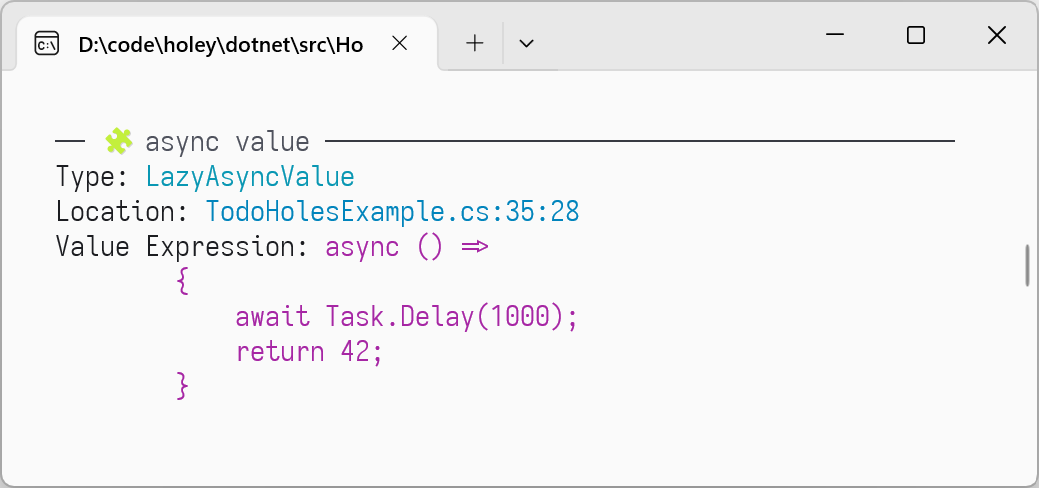
\includegraphics[width=0.9\textwidth]{images/cli-reporting}
    \caption{TODO}
    \label{fig:holey-cli-reporting}
\end{figure}

Figure~\ref{fig:holey-cli-reporting} shows how such a custom reporter can look like.
In this case, the application using Holey is a command line application and a reporter is registered that formats the type, location and expression of side effect holes and prints it to the console.
This highlights if a hole is executed at runtime.
Holey enables custom reporters to be registered for the following events:
\begin{description}
    \item[Hole Encountered] Before a hole is executed, it gets encountered. This event provides all the information gathered about the hole during runtime and compile time. Figure~\ref{fig:holey-cli-reporting} depicts this kind of event.
    \item[Value Provided] Reporters can be registered if values are provided. In addition to the hole's information this event also provides information about the provided value.
    \item[Async Value Provided] When a value is provided asynchronously, the following events can be analyzed: started, completed, faulted, and canceled.
    \item[Effect Happened] Analogous to provided values, reporters enable the visualization of executed effects. In comparison the provided values, effects provide no return value, hence this event only reports information about the hole.
    \item[Async Effect Happened] Similar to async values, the following events of async effects can be reported: started, completed, faulted, and canceled.
\end{description}
Figure~\ref{fig:holey-sidecar} in Section~\ref{sec:holey-sidecar} shows a more complex scenario of utilizing Holey's reporters.
The bottom left pane reports all previously mentioned events.
Supplied values are displayed as collapsable JSON objects while asynchronous values and effects automatically update their list entries with the async state.
This example also demonstrates that reporting holes is not limited to the application itself, but can be done in an additional application connected to the application under development (e.g., an IDE plug-in).

\subsection{Fake Data Generation}
\label{sec:holey-fake-data-generation}
As side effect holes are incomplete parts of a program which can provide some temporary behavior, they can be perfectly complemented by fake data generators.
Providing temporary data or behavior via holes gives the following advantages:
\begin{itemize}
    \item By not necessarily relying on constant values the programs behavior is more similar to the real world.
    \item Because of the compile time support for holes, these incomplete parts of the program can be found easier later on.
    \item These implementations can be re-used, e.g., as inputs for test cases.
\end{itemize}

After we simplified side effect holes to simply return a value or return an effect (with their respective lazy and asynchronous counterparts) we realized that we gained support for all standard faking and mocking libraries by providing such a simple interface.
If one thinks of the responsibilities of fake data generation libraries or mocking and stubbing libraries, they are mainly used for the arrange phase of tests.
They either provide some test data or mock an interface to test against.
\emph{Test-Driven Development} (TDD) is a perfect fit for specified requirements, but as soon as process of creating software involves more ideation and prototyping phases, the rigid structure of TDD can hinder development.

Holey's approach on Hole-Driven Development allows developers to use the same tools (e.g. Bogus\footnote{\url{https://github.com/bchavez/Bogus}} or NSubstitute\footnote{\url{https://nsubstitute.github.io/}} known from TDD to use for prototyping.
Program~\ref{prg:holey-supporting-mocking-libraries} shows the usage of the fake data generation libraries Bogus and AutoBogus\footnote{\url{https://github.com/nickdodd79/AutoBogus}} to provide dynamic values in side effect holes.
While in the first example showcasing Bogus, developers have to specify rules for generating properties by hand, the second example shows how AutoBogus is capable of automatically generating an instance of the record \texttt{User} by applying heuristics based on the property names and types.
While the latter automatic mode of generating test data is extremely comfortable and concise, it lacks the parametrization capabilities and authenticity of manually specifying rules for dummy data generation.

By using Holey's sidecar application (compare Section~\ref{sec:holey-sidecar}), developers and users can specify dummy data at runtime via an external application; thus it enables them to simulate the real world even more genuine.

\begin{program}[ht]
\begin{CsCode}
// === Bogus ===
private static readonly Faker faker = new("en");
internal record Weather(int Celsius, float Humidity, string Description);
var weather = Hole.Todo(
	"get the weather from a weather service",
	() =>
		new Weather(
			Celsius: faker.Random.Number(-20, 40),
			Humidity: faker.Random.Float(20, 99.9f),
			Description: faker.PickRandom("sunny", "cloudy", "rainy")
		)
);

// === AutoBogus ===
AutoFaker.Configure(builder => builder.WithConventions());
internal record User(Guid Id, string FirstName, string LastName, string EMail);
var user = Hole.Todo(
    "load the user from the database",
    () => AutoFaker.Generate<User>()
);
\end{CsCode}
\caption{Using the libraries Bogus and AutoBogus to generate fake data for side effect holes.}
\label{prg:holey-supporting-mocking-libraries}
\end{program}

\subsection{Sidecar Application}
\label{sec:holey-sidecar}
An extension we developed to show the capabilities of Holey's extension system is the Sidecar application\footnote{A hosted version of the Sidecar is available at \url{https://sidecar.holey.dev}, but it can also be self-hosted as it is a static web app.}.
This application is not directly built into Holey, but solely built on its extension capabilities such as reporters, querying all existing holes and extending side effect holes.
Its name \emph{Sidecar} is inspired by sidecar pattern of microservice architectures, which allow an additional application to be attached to a parent application which provides supporting features \cite{microsoft_sidecar_nodate}.
An example of using this extension is shown in Program~\ref{prg:holey-sidecar-prompting}.
Line~\verb|1| adds the using needed for supporting prompting for values via the Sidecar application.
After adding this using, one can use the extension method \texttt{\seqsplit{Prompt<T>()}} to prompt for a value of type \verb|T|.
This method pauses the application and uses the \emph{json-everything}\footnote{\url{https://json-everything.net}} library to create a JSON Schema based on the type passed to \texttt{\seqsplit{Prompt<T>()}} via the generic type parameter.
%
\begin{program}[ht]
\begin{CsCode}
using Holey.Extension.Sidecar.Logic.Prompting;
internal record Weather(
	[property: Required] int Celsius,
	[property: Required] float Humidity,
	[property: Required] string Description
);
var weather = Hole.Todo(
	"prompt the user for the weather",
	value => value.Prompt<Weather>()
);
\end{CsCode}
\caption{Usage of Holey's Sidecar Extension to interactively prompt a Value.}
\label{prg:holey-sidecar-prompting}
\end{program}
%
This JSON Schema is then sent to the Sidecar application which renders a form using \emph{react-jsonschema-form}\footnote{\url{https://github.com/rjsf-team/react-jsonschema-form}}.
The result of this process can be seen in the bottom right pane of Figure~\ref{fig:holey-sidecar}.
Once again, by building a composable library and using composable libraries we managed to convert a type to a JSON Schema in one line of code and render the form in another one.
Now the user of the Sidecar application can enter the desired values (\ref{hp:visually-editable}) which get sent back to the parent application and temporarily act as the hole's value.
The small crystal ball to the right of the form's title tries to magically auto-fill the form and can be used to speed-up testing.
It follows the same concept as AutoBogus (compare Section~\ref{sec:holey-fake-data-generation}) but is based on the JavaScript library \emph{json-schema-faker}\footnote{\url{https://github.com/json-schema-faker/json-schema-faker}}.
As this data generation is conducted on the client, Hole-Driven Development libraries for other languages would automatically benefit from this feature as well.

One aspect of developing the Sidecar application was keeping it as independent as possible.
Multiple applications can connect at the same time, their programming languages do not affect the Sidecar and it can be connected in multiple ways.
For this thesis we showed that it can be connected via Websockets on the local network, via proxied Websockets via PartyKit\footnote{\url{https://www.partykit.io}} and via iFrames using \texttt{\seqsplit{postMessage}} as its communication channel.
These communication channels can also be mixed and matched and are passed to the Sidecar application via URL params as shown in the address bar of Figure~\ref{fig:holey-sidecar}.

\begin{figure}[ht]
    \centering
    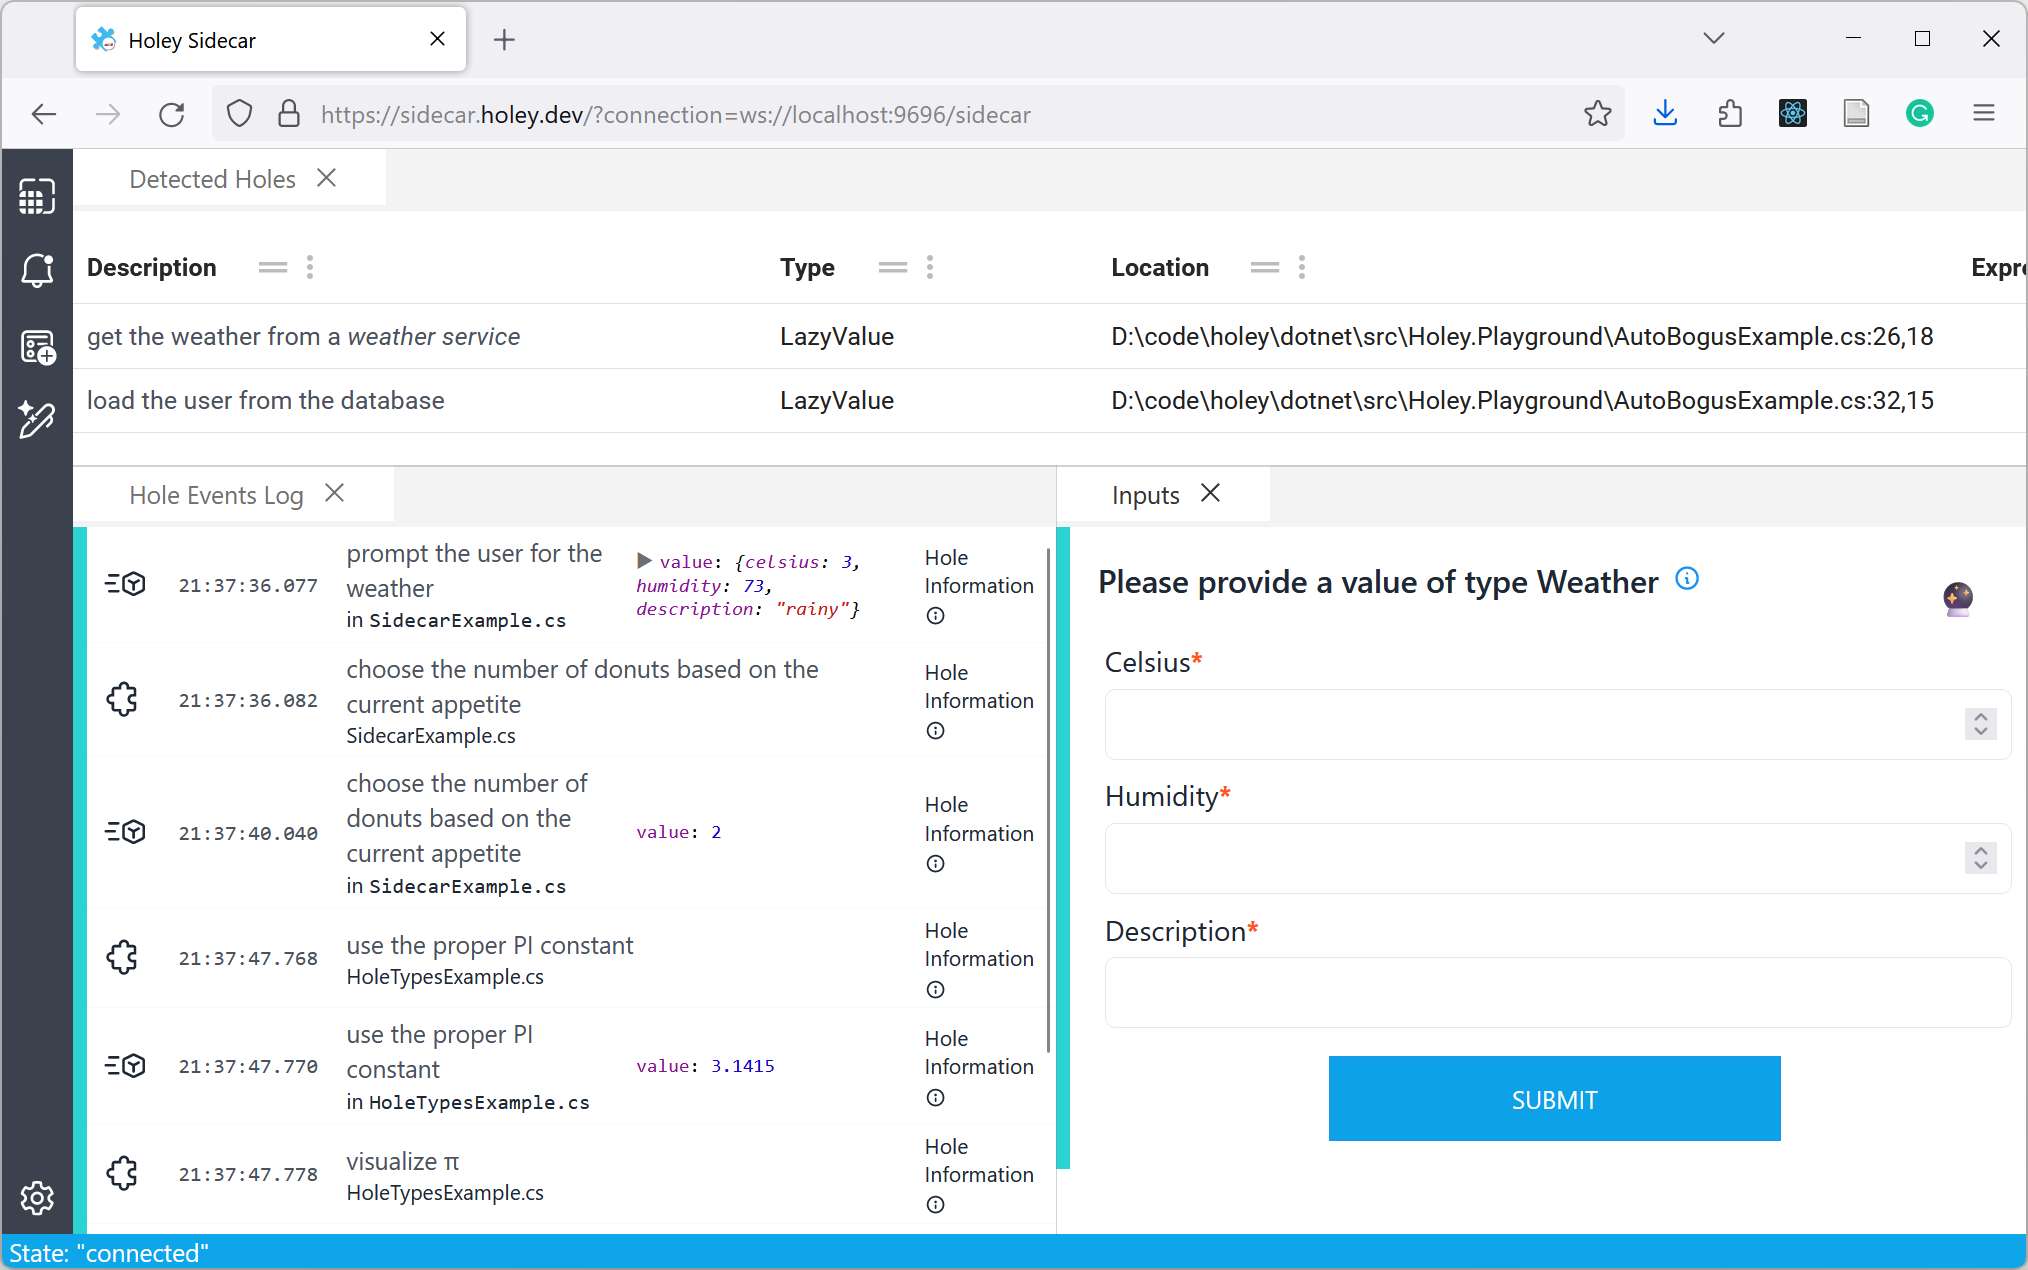
\includegraphics[width=0.9\textwidth]{images/sidecar}
    \caption{Holey Sidecar Application listing discovered Holes, Hole interactions and a dynamically rendered Form for prompting the Weather.}
    \label{fig:holey-sidecar}
\end{figure}